%%%%%%%%%%%%%%%%%%%%%%%%%%%%%%%%%%%%%%%%%
% Beamer Presentation
% LaTeX Template
% Version 1.0 (10/11/12)
%
% This template has been downloaded from:
% http://www.LaTeXTemplates.com
%
% License:
% CC BY-NC-SA 3.0 (http://creativecommons.org/licenses/by-nc-sa/3.0/)
%
%%%%%%%%%%%%%%%%%%%%%%%%%%%%%%%%%%%%%%%%%

\documentclass[t]{beamer}

\usepackage[english]{babel}
\usepackage[utf8]{inputenc}
\usepackage{hyperref}
\usepackage{verbatim}
\usepackage{listings}

%----------------------------------------------------------------------------------------
%	PACKAGES AND THEMES
%----------------------------------------------------------------------------------------

\mode<presentation> {

% The Beamer class comes with a number of default slide themes
% which change the colors and layouts of slides. Below this is a list
% of all the themes, uncomment each in turn to see what they look like.

%\usetheme{default}
%\usetheme{AnnArbor}
%\usetheme{Antibes}
%\usetheme{Bergen}
%\usetheme{Berkeley}
%\usetheme{Berlin}
%\usetheme{Boadilla}
%\usetheme{CambridgeUS}
%\usetheme{Copenhagen}
%\usetheme{Darmstadt}
%\usetheme{Dresden}
%\usetheme{Frankfurt}
%\usetheme{Goettingen}
%\usetheme{Hannover}
%\usetheme{Ilmenau}
%\usetheme{JuanLesPins}
%\usetheme{Luebeck}
%\usetheme{Madrid}
%\usetheme{Malmoe}
%\usetheme{Marburg}
%\usetheme{Montpellier}
%\usetheme{PaloAlto}
%\usetheme{Pittsburgh}
%\usetheme{Rochester}
%\usetheme{Singapore}
%\usetheme{Szeged}
\usetheme{Warsaw}

% As well as themes, the Beamer class has a number of color themes
% for any slide theme. Uncomment each of these in turn to see how it
% changes the colors of your current slide theme.

%\usecolortheme{albatross}
%\usecolortheme{beaver}
%\usecolortheme{beetle}
%\usecolortheme{crane}
%\usecolortheme{dolphin}
%\usecolortheme{dove}
%\usecolortheme{fly}
%\usecolortheme{lily}
%\usecolortheme{orchid}
%\usecolortheme{rose}
\usecolortheme{seagull}
%\usecolortheme{seahorse}
%\usecolortheme{whale}
%\usecolortheme{wolverine}

\usefonttheme{structuresmallcapsserif}

%\setbeamertemplate{footline} % To remove the footer line in all slides uncomment this line
%\setbeamertemplate{footline}[page number] % To replace the footer line in all slides with a simple slide count uncomment this line

%\setbeamertemplate{navigation symbols}{} % To remove the navigation symbols from the bottom of all slides uncomment this line
}


\usepackage{graphicx} % Allows including images
\usepackage{booktabs} % Allows the use of \toprule, \midrule and \bottomrule in tables



\lstdefinestyle{cpp}{
  language=C++,
  basicstyle=\ttfamily\footnotesize,  % Use small true type font
  showstringspaces=false,                 % Don't put marks in string spaces
  tabsize=2,                              % 5 spaces per tab
  escapeinside={@}{@},                % for invisible labels
  breaklines=true,
  breakatwhitespace=true,
  emptylines=1,
  texcl=true,
  escapechar=@,
  mathescape=true,
  xleftmargin=2.5ex,
  keywordstyle=[1]\color{blue},
  % keywordstyle=[2]\color{red},
	% stringstyle=\color{red},
	% commentstyle=\color{green},
	% morekeywords=[1]{pop_front}
	% morekeywords=[2]{parent,child}
}


\author[]{Kevin Wallimann \quad Johannes Baum \quad Matthias Untergassmair}

%----------------------------------------------------------------------------------------
%	TITLE PAGE
%----------------------------------------------------------------------------------------

\title[Topological Sorting]{Parallel Topological Sorting} % The short title appears at the bottom of every slide, the full title is only on the title page
\subtitle{Design of High Performance Computing, Fall 2015}

\institute[ETHZ]{ ETH Zürich }
%\date{\today} % Date, can be changed to a custom date
\date{December 14, 2015}
	\begin{document}

\begin{frame}
\titlepage % Print the title page as the first slide
\end{frame}

%----------------------------------------------------------------------------------------
%	PRESENTATION SLIDES
%----------------------------------------------------------------------------------------

%------------------------------------------------
\section{Overview}
%------------------------------------------------


\begin{frame}
\frametitle{Overview}

\begin{itemize}
\item DAG defines partial order
\item Topological sorting defines one total order on a DAG
\item Parallel algorithm: finds one topological sorting of a given DAG
\end{itemize}

\end{frame}

%------------------------------------------------
\section{Difference to BFS}
%------------------------------------------------

\begin{frame}
\frametitle{Difference to BFS}

\begin{itemize}
\item BFS visits every node
\item Topological sorting algorithm needs to visit every edge
\item Thus no BFS optimizations like bottom-up-BFS possible
\end{itemize}

Example:

\begin{figure}[!hbp]
 
  \begin{tikzpicture}[->,>=stealth',auto,node distance=1cm,
                    thick,main
                    node/.style={circle,draw,font=\sffamily\scriptsize},text node/.style={draw=none,font=\sffamily\tiny}]

  \node[main node] (1) [draw=black!80,text=black!80] {A};
  \node[main node] (2) [below right of=1, node distance=1.2cm]{B};
  \node[main node] (3) [below of=1, node distance=1.2cm] {C};
  

  \path[every node/.style={font=\sffamily\small}]
    (1) edge (2)
    (2) edge (3)
    (1) edge (3)
    ;
\end{tikzpicture}

\end{figure}

Consider order A,C,B
$\rightarrow$ valid in BFS, invalid in topological sorting


\end{frame}

%------------------------------------------------
\section{Input graphs}
%------------------------------------------------

\begin{frame}
\frametitle{Random graph}
\begin{figure}[!hbp]
    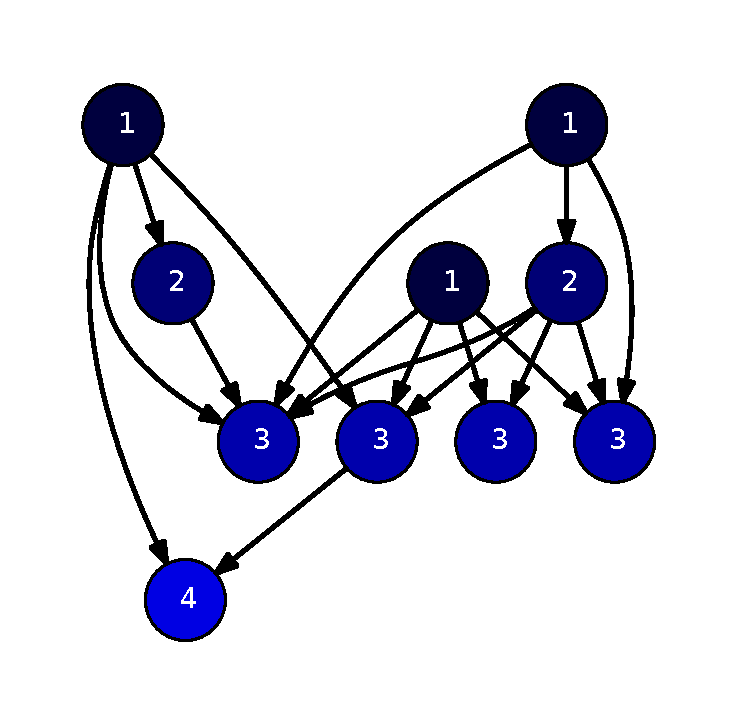
\includegraphics[height=0.7\textheight]{img/random_lin10.pdf}
\end{figure}

\end{frame}

\begin{frame}
\frametitle{Software dependency graph}
\begin{figure}[!hbp]
    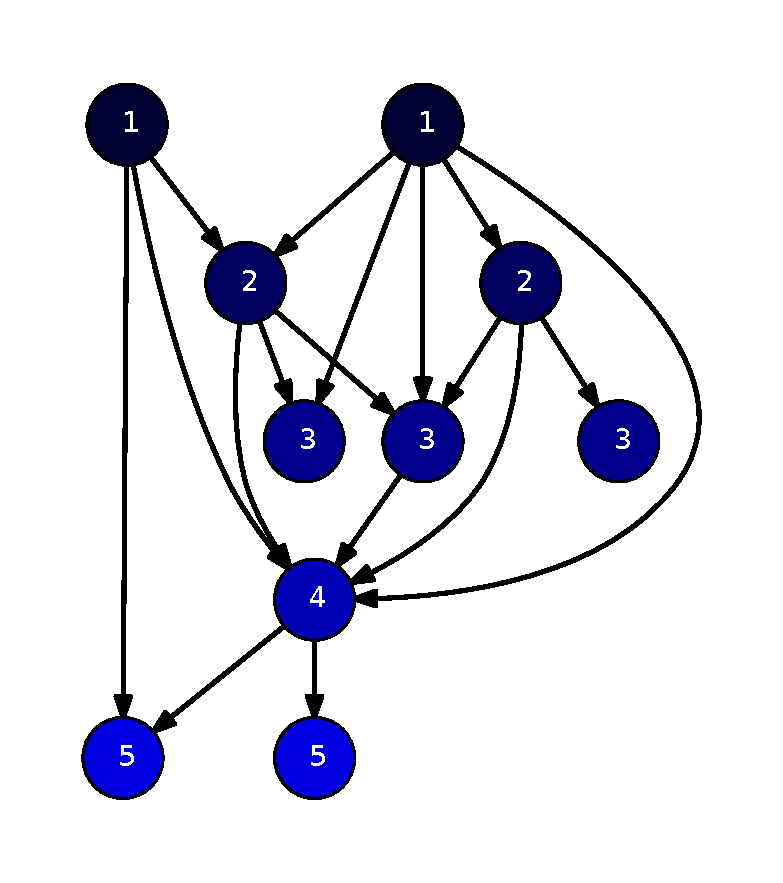
\includegraphics[height=0.7\textheight]{img/software10.pdf}

\end{figure}
{\color{gray}\tiny Musco, V. et al. (2014) "A Generative Model of Software Dependency Graphs to Better Understand Software Evolution."}
\end{frame}


%------------------------------------------------
\section{Implementations}
%------------------------------------------------

\begin{frame}
\frametitle{Implementations}

List based approach:
\begin{itemize}
\item Nodes to be visited ("front") are stored in a linked list
\item Every thread builds its local list
\item Local lists are merged and redistributed at synchronization points to distribute work equally
\end{itemize}

Array based approach:
\begin{itemize}
\item Nodes to be visited are stored in a global bytemap which maps the node id to a boolean value
\end{itemize}

\end{frame}

%------------------------------------------------
\section{Results}
%------------------------------------------------

\begin{frame}
\frametitle{Results - Xeon Phi}



\end{frame}


\end{document} 
